\documentclass[12pt]{article}
\usepackage[spanish, english, es-tabla]{babel}
\usepackage[utf8]{inputenc}
\usepackage[left = 2cm, right = 2cm, bottom = 2cm, top = 3cm]{geometry}
\usepackage{amsmath, amssymb}
\usepackage{graphicx}
\usepackage{hyperref}

\begin{document}
    \selectlanguage{spanish}
    \title{DPDK y Openflow-OKO \\ \large Trabajo Final de Estudios}
    \author{Enrique Fernández Sánchez}
    
    %% EDITAR PARA SEGUIMIENTO DE VERSIONES
    \date{Revisión 19 Febrero 2021}
    
    \maketitle
    \tableofcontents
    
    \pagebreak

    %%% TODO
    \section{Introduction}
    
    \pagebreak
    
    \section{DPDK}
    \subsection{¿Qué es?}
    DPDK (\emph{Data Plane Development Kit}) es un proyecto Open Source controlado por la Fundación Linux. Dicho proyecto tiene por objetivo proveer unas librerías de "plano de datos" y controladores para comunicarse con los propios controladores de las interfaces de red, con la finalidad de descargar el procesamiento de los paquetes TCP/UDP desde el núcleo del sistema operativo a los diferentes procesos que se ejecutan en el espacio de usuario (aplicaciones). Con esta descarga, lo que conseguimos es liberar al procesador de ciertas tareas especificas, dando por resultado una mayor eficiencia informática y un mayor rendimiento de paquetes, ya que introducimos mejoras a las propias instrucciones que nos proporciona el kernel.\\
    
    \noindent \emph{Data Plane Development Kit} surge a una alternativa competitiva para el procesamiento de paquetes de red. Si bien es cierto que actualmente el procesado que hace Linux de los paquetes es bastante eficiente, con DPDK podemos llevar a incrementar muchísimo la velocidad de procesado. Esto es muy importante ya que de cara a tecnologías futuras, comunicaciones de fibra óptica o el 5G, es muy necesario que los servidores del backbone, o aplicaciones específicas de routers y switches, puedan responder a las grandes necesidades que se nos proponen.\\
    
    \begin{figure}[h]
        \begin{center}
        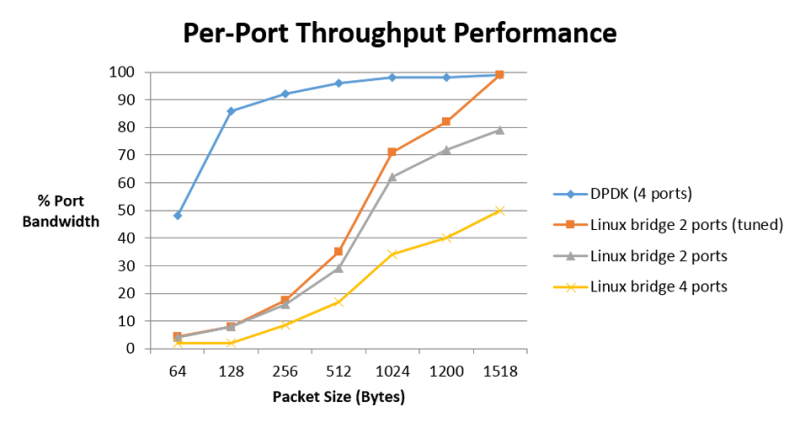
\includegraphics[width=1\textwidth]{img/TB_per-port-throughput-performance-800x428.png}
        \caption{Comparación entre Linux y DPDK. (\ref{bib:img 1})}
        \end{center}
    \end{figure}
    
    \pagebreak
    
    \subsection{Requisitos para utilizar DPDK.}
    
    
    
    \subsection{¿Qué son las Huge Page?}
    
    
    
    %%% Bibliography
    \pagebreak
    \section{Bibliografía}
    \hyperref[bib:link1]{\emph{Reference of bibliography}}
    \begin{enumerate}
        %1
        \item \label{bib:link1} \href{https://blog.selectel.com/introduction-dpdk-architecture-principles/}{Introduction to DPDK: Architecture and Principles}
        
        %2
        \item \label{bib:link2}\href{https://en.wikipedia.org/wiki/Data_Plane_Development_Kit}{Wikipedia: Data Plane Development Kit}
        
        %3
        \item \label{bib:img1}\href{https://www.accton.com/Technology-Brief/intel-dpdk-performance-on-the-sau5081i-server/}{Imagen comparativa de BW en diferentes tests case.}
        
        %4
        \item \label{bib:link3}\href{https://wiki.debian.org/Hugepages}{Hugepages}
    \end{enumerate}
\end{document}